\documentclass[10pt]{beamer}

\usetheme[progressbar=frametitle]{metropolis}
\usepackage{appendixnumberbeamer}

\usepackage{booktabs}
\usepackage[scale=2]{ccicons}

\usepackage{pgfplots}
\usepackage{graphicx}
\usepgfplotslibrary{dateplot}

\usepackage{xspace}
\newcommand{\themename}{\textbf{\textsc{metropolis}}\xspace}
\graphicspath{ {./img/} }

\title{Computational Social Science \& Humanities}
\subtitle{A cold take by a self-taught dabbler in computational methods and techniques}
\date{December 8th 2022}
\author{Kristian G. Kjelmann}
\institute{Department of Sociology \& Social Work}
% \titlegraphic{\hfill\includegraphics[height=1.5cm]{logo.pdf}}

\begin{document}

\maketitle

%\begin{frame}{Table of contents}
%  \setbeamertemplate{section in toc}[sections numbered]
%  \tableofcontents%[hideallsubsections]
%\end{frame}

\section{What is CSSH seen from your perspective?}

\begin{frame}[fragile]{What it is not}

    \begin{itemize}
        \item Anything involving large amounts of data
        \item Anything "beyond" econometrics
        \item Anything involving programming
    \end{itemize}
  
\end{frame}

\begin{frame}[fragile]{What it is}

\begin{quote}
    Techniques for \alert{condensing}, \alert{making sense of} or \alert{deriving meaningful measurements} from \alert{high dimensional} and (mainly) \alert{unstructured data} 
\end{quote}

    \begin{itemize}[<+- | alert@+>]
        \item Exploratory
        \item Experimental
        \item Complimentary
        \item Integrated (in research domain)
    \end{itemize}
  
\end{frame}

\begin{frame}[fragile]{My areas of interest}

    Generally: \emph{Changes and variations in societal discourses}
    \begin{itemize}
        \item The legitimization and de-legitimization of views and opinions
        \item Emergence and manifestation of hegemonic discourses
        \item In- and outgroup dynamics as expressed in speech
        \item Interplay of societal developments and discourses on societal developments
    \end{itemize}

    Specifically (currently): \emph{Co-variation in discourses and ethnic integration outcomes at local community levels}
    
\end{frame}

\section{How could you and your group benefit from a CSSH Hub?}

\begin{frame}[fragile]{Discussing methods and techniques}  
\begin{columns}[T,onlytextwidth]
    \column{0.50\textwidth}
        \centering
        Me
        
        
\includegraphics[width=0.95\textwidth]{excited}

\end{columns}


\end{frame}

\begin{frame}[fragile]{Discussing methods and techniques}  
\begin{columns}[T,onlytextwidth]
    \column{0.50\textwidth}
        \centering
        Me
        
        
\includegraphics[width=0.95\textwidth]{excited}
    \column{0.50\textwidth}
        \centering
        My colleagues
        
        
\includegraphics[width=0.95\textwidth]{confused}

\end{columns}


\end{frame}

\begin{frame}[fragile]{Unpacking the black boxes}  
    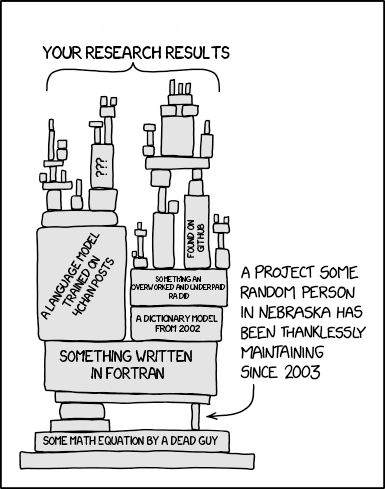
\includegraphics[scale=0.4]{dependency_cssh}
    \centering
    
    \textit{Adapted from:} \href{https://xkcd.com/2347/}{\textit{https://xkcd.com/2347/}}.
    \centering

\end{frame}

\begin{frame}[fragile]{Navigating the tools}  
\begin{columns}[T,onlytextwidth]
    \column{0.50\textwidth}
        \centering
        What I know
        
        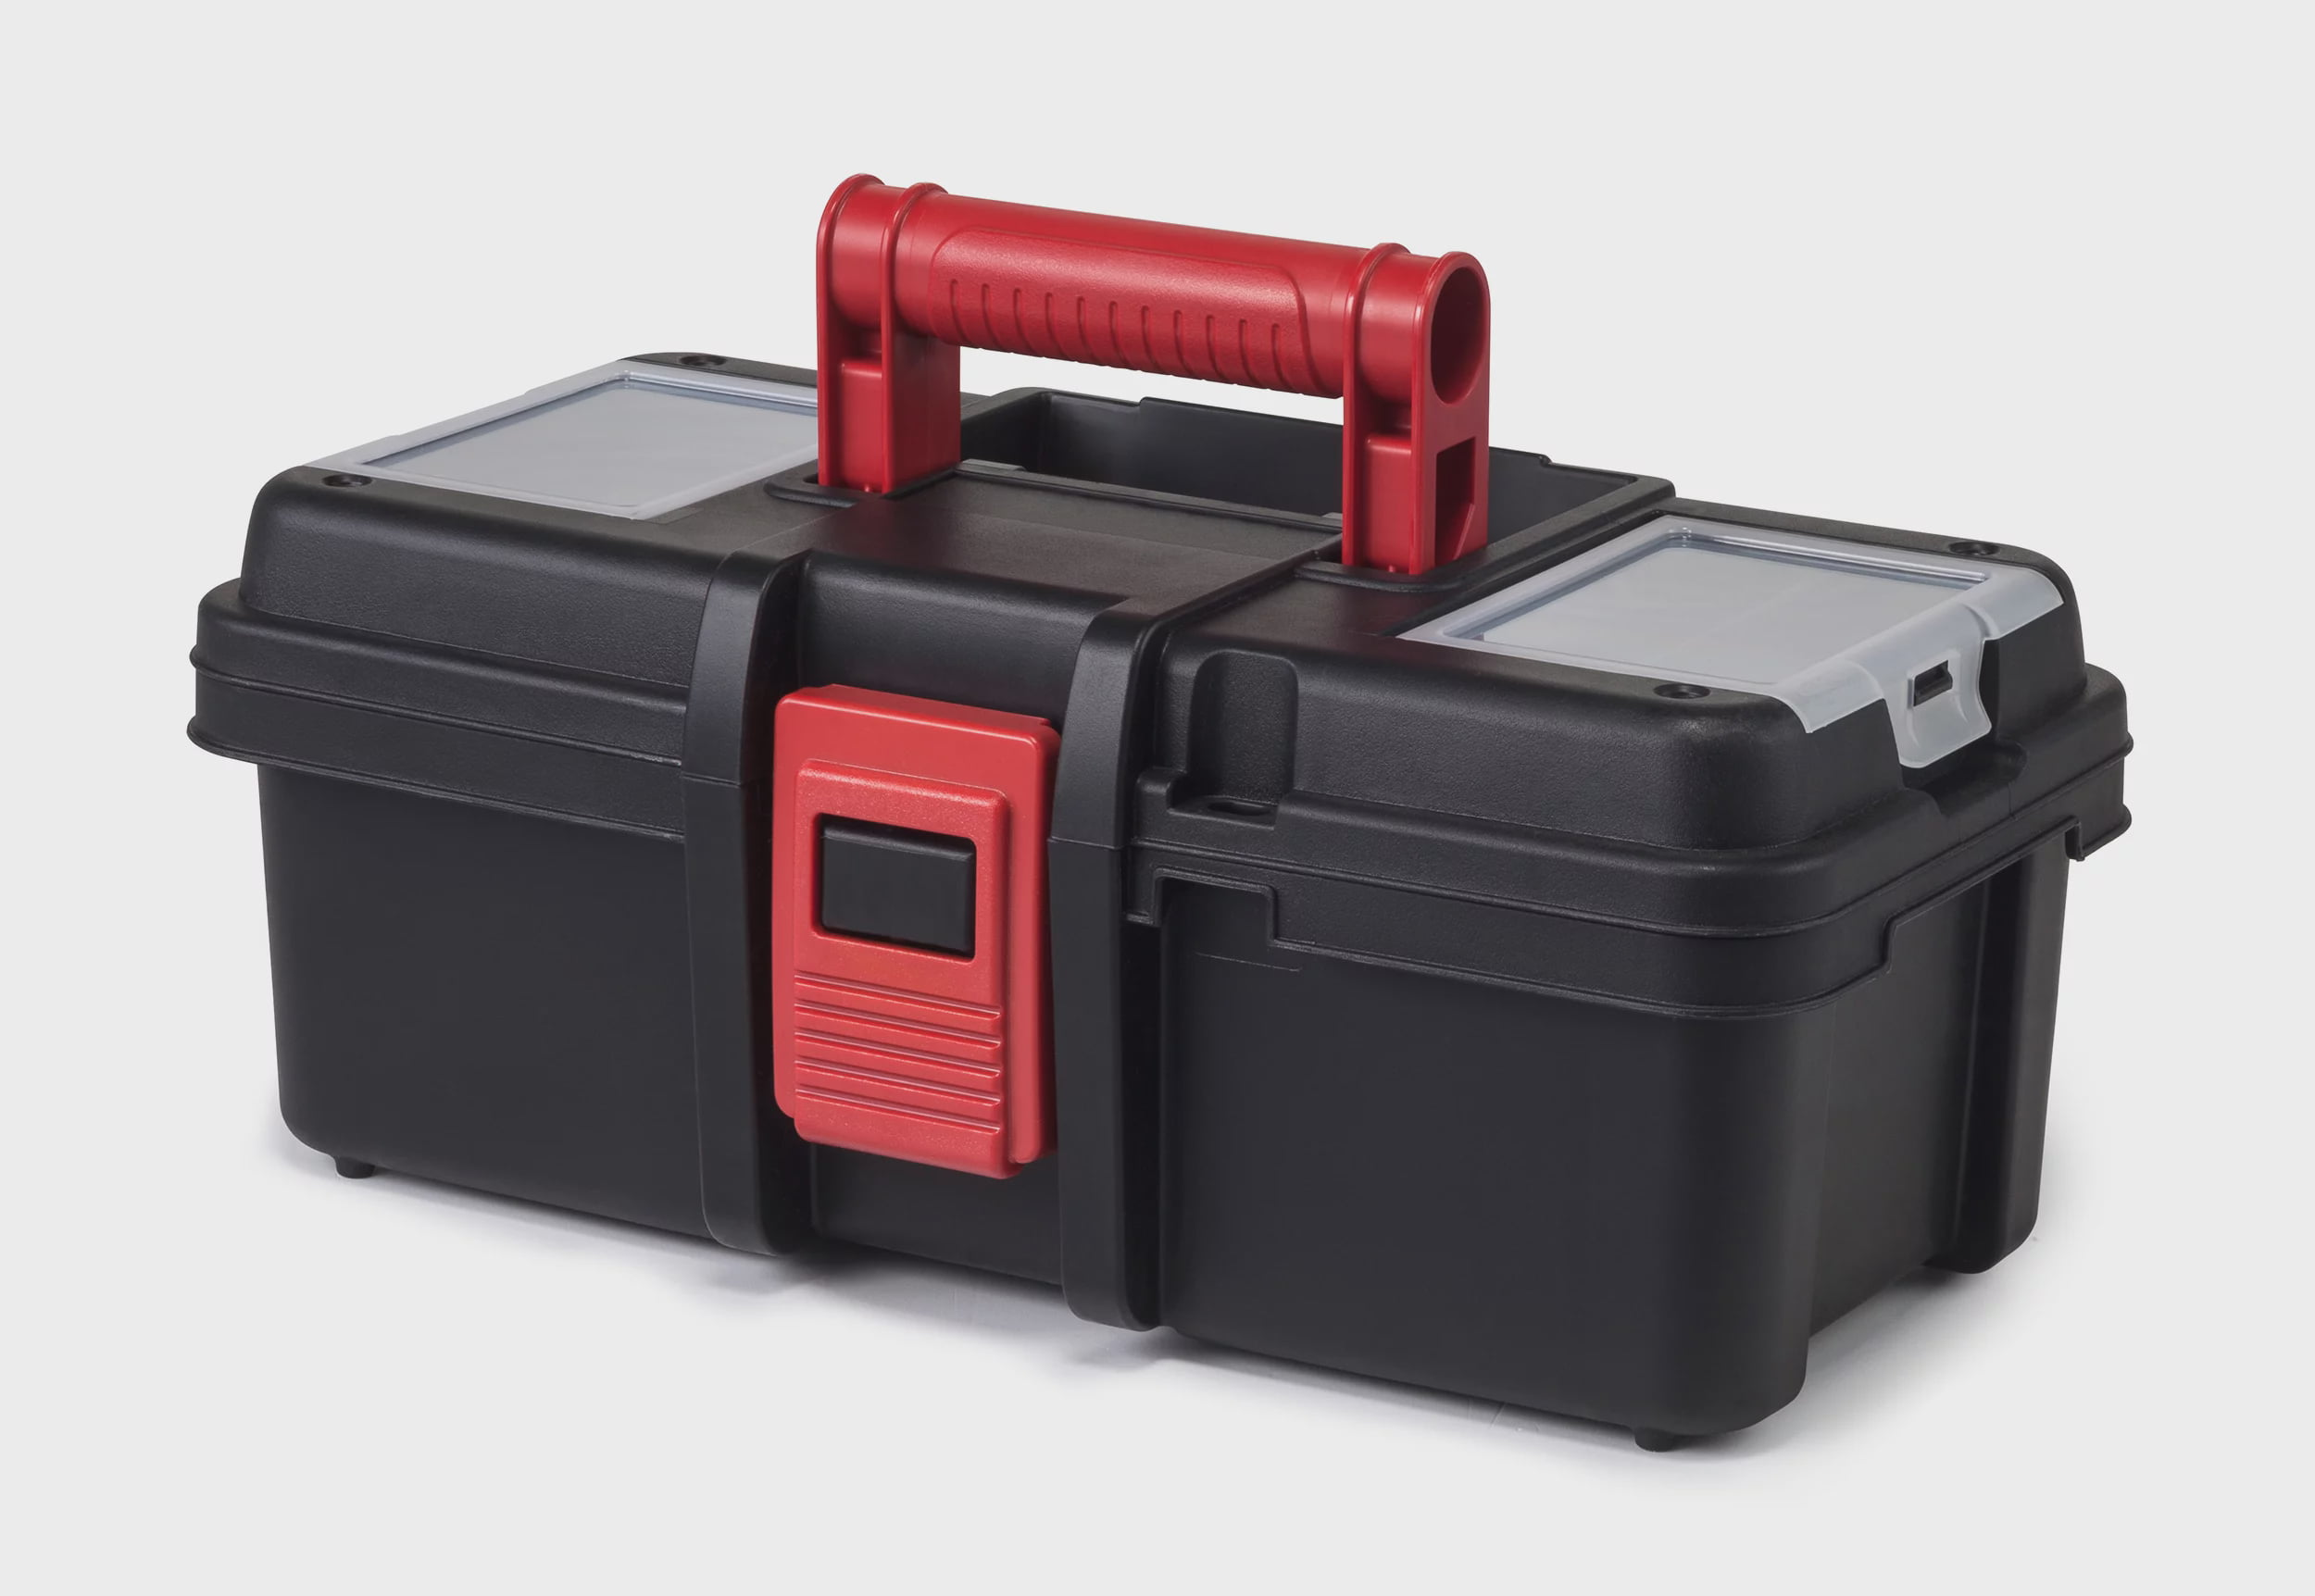
\includegraphics[width=0.95\textwidth]{toolbox}
    \column{0.50\textwidth}
        \centering
        What is available
        
        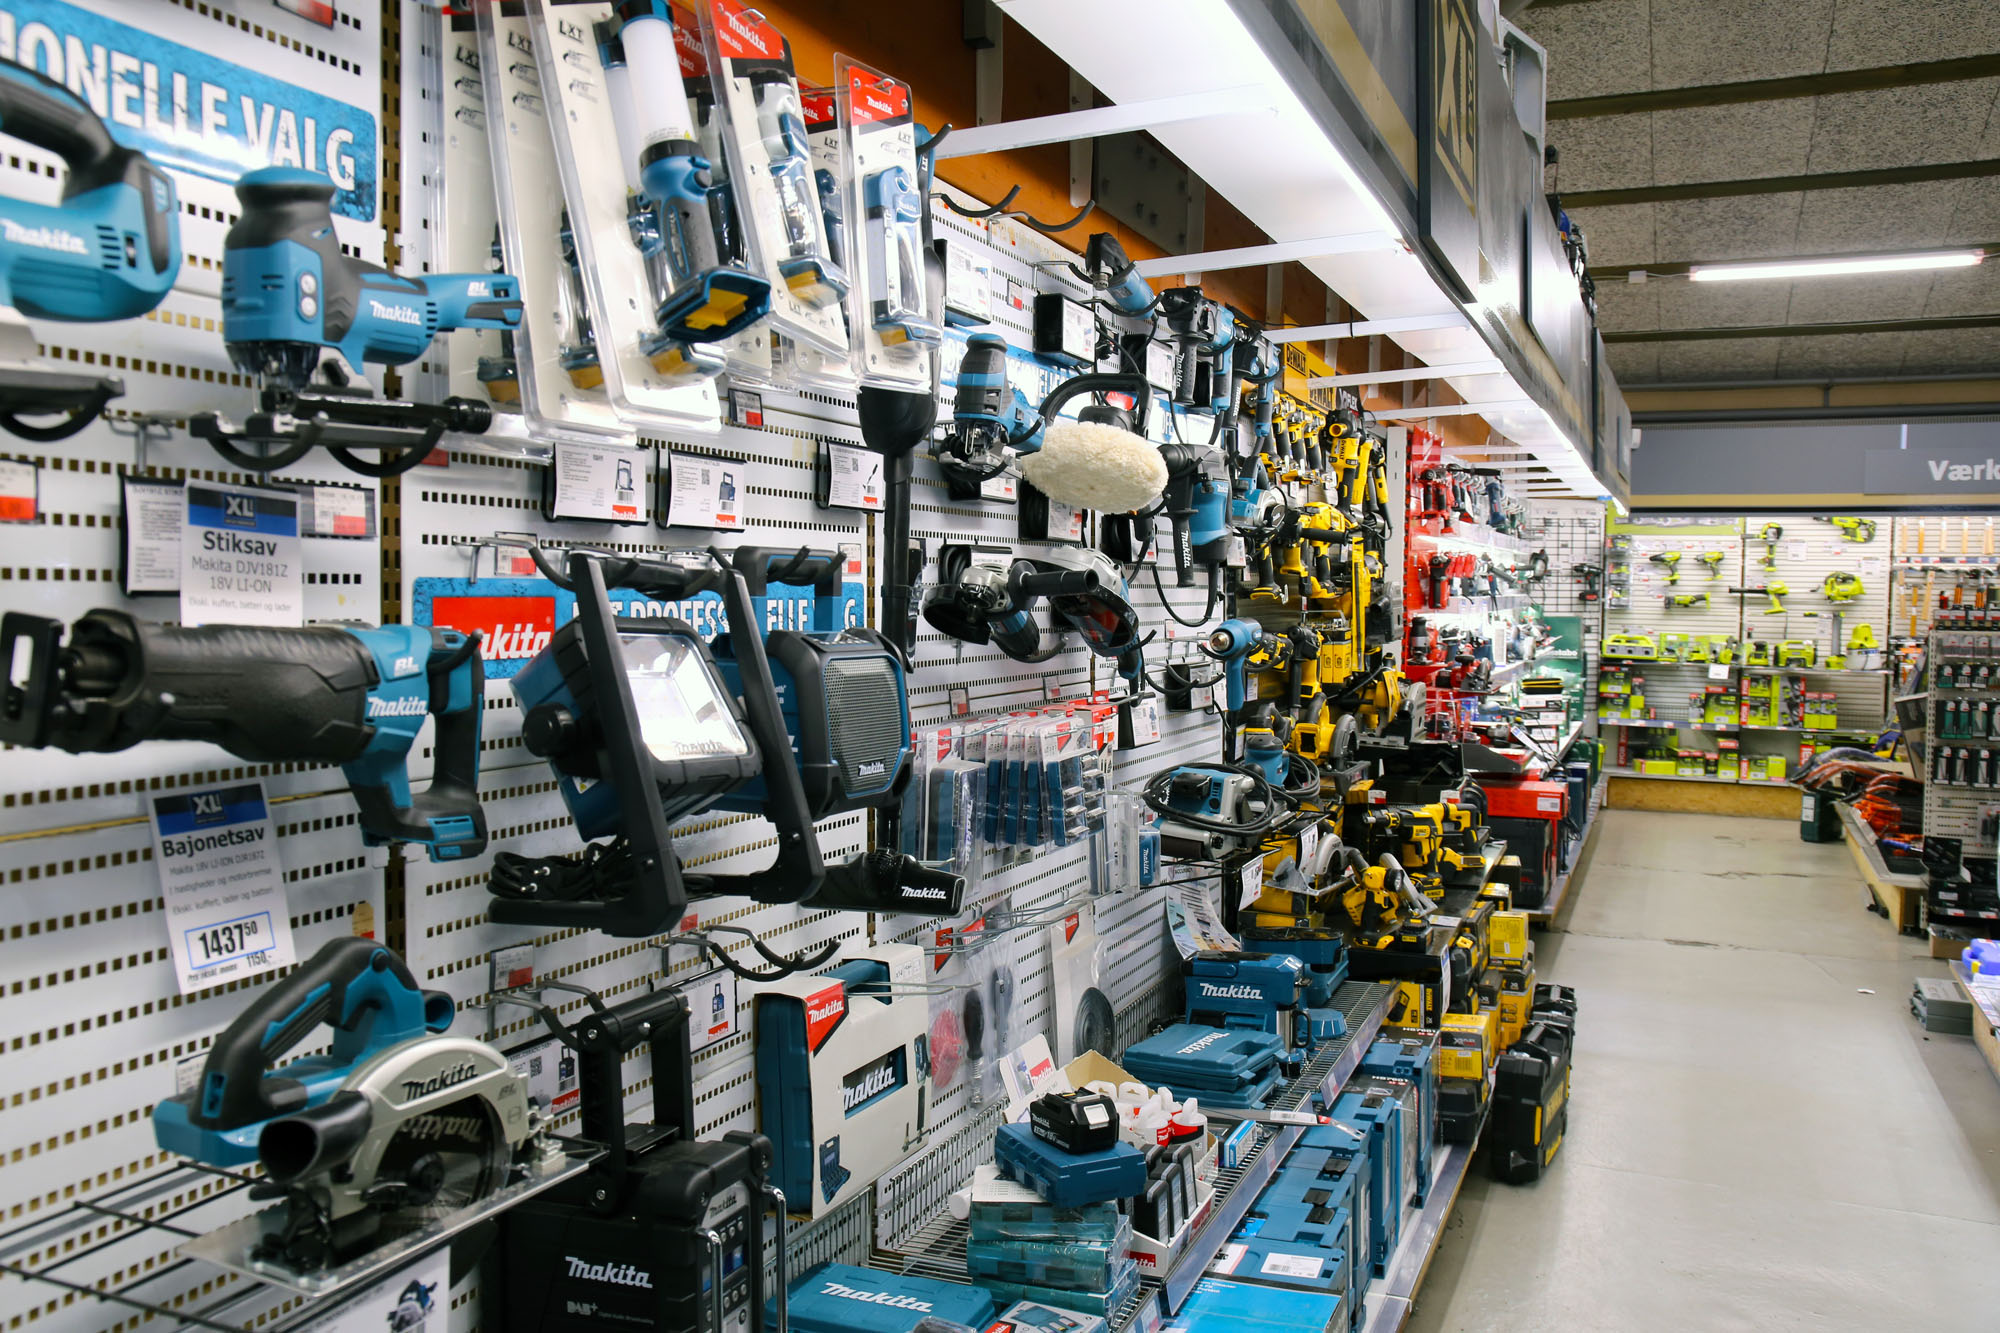
\includegraphics[width=0.95\textwidth]{byggemarked}

\end{columns}


\end{frame}

\section{Where do you picture that CSSH will be at AAU in three years?}

\begin{frame}{From novel approaches...}

    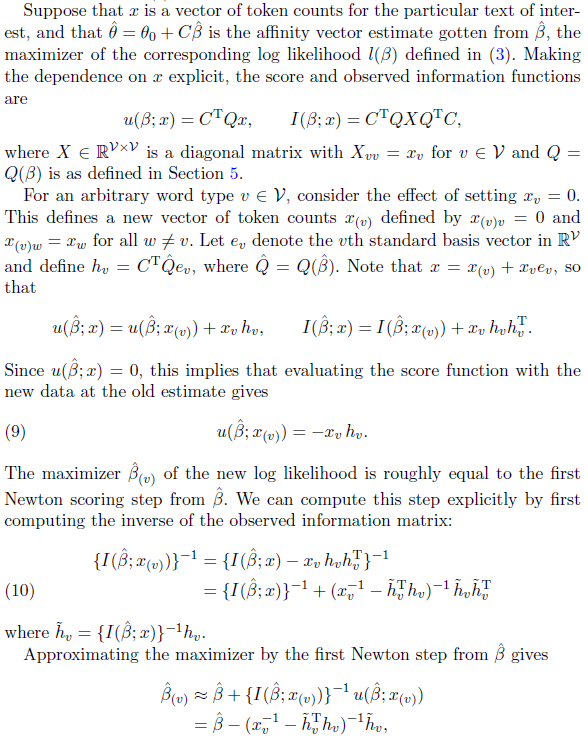
\includegraphics[height=0.9\textheight]{formula-heavy}
    \centering
%    \begin{figure}[!h]
%        \centering
%        $\vcenter{\hbox{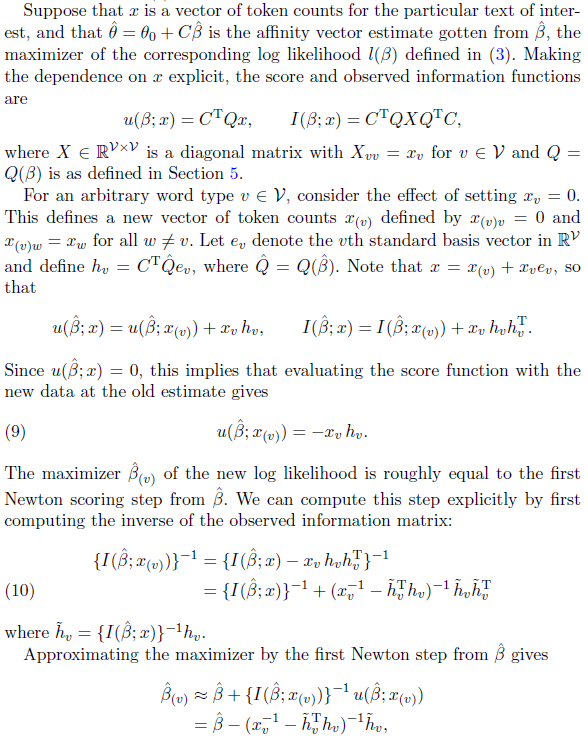
\includegraphics[width=0.45\textwidth]{formula-heavy}}}$
%        \qquad
%        $\vcenter{\hbox{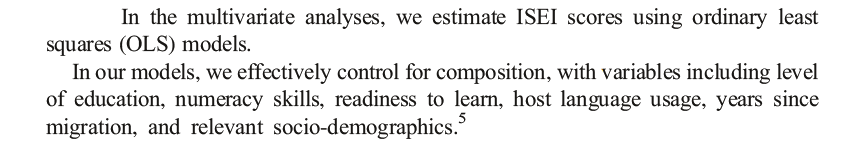
\includegraphics[width=0.45\textwidth]{formula-none}}}$
%        \qquad
%    \end{figure}

\end{frame}

\begin{frame}{...to established conventions}

    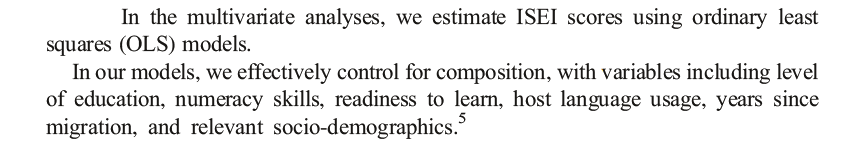
\includegraphics[width=\textwidth]{formula-none}
    \centering

\end{frame}


\begin{frame}[fragile]{From single to team authorship}  
    
    
\includegraphics[width=\textwidth]{single-multiple}
    \centering

\end{frame}

\begin{frame}{(Co-)Developed tools}

    
\includegraphics[width=0.8\textwidth]{tools-cssh}
    \centering
    
\end{frame}
\end{document}